In order to judge different performance measures of our final model, we require a baseline.
Such a baseline needs to align to the collection of tasks described in Section~\ref{sec:introduction} as close as
possible to allow for good comparability of results.

\begin{wrapfigure}{r}{0.4\textwidth}
    \centering
    \vspace{-10pt}
    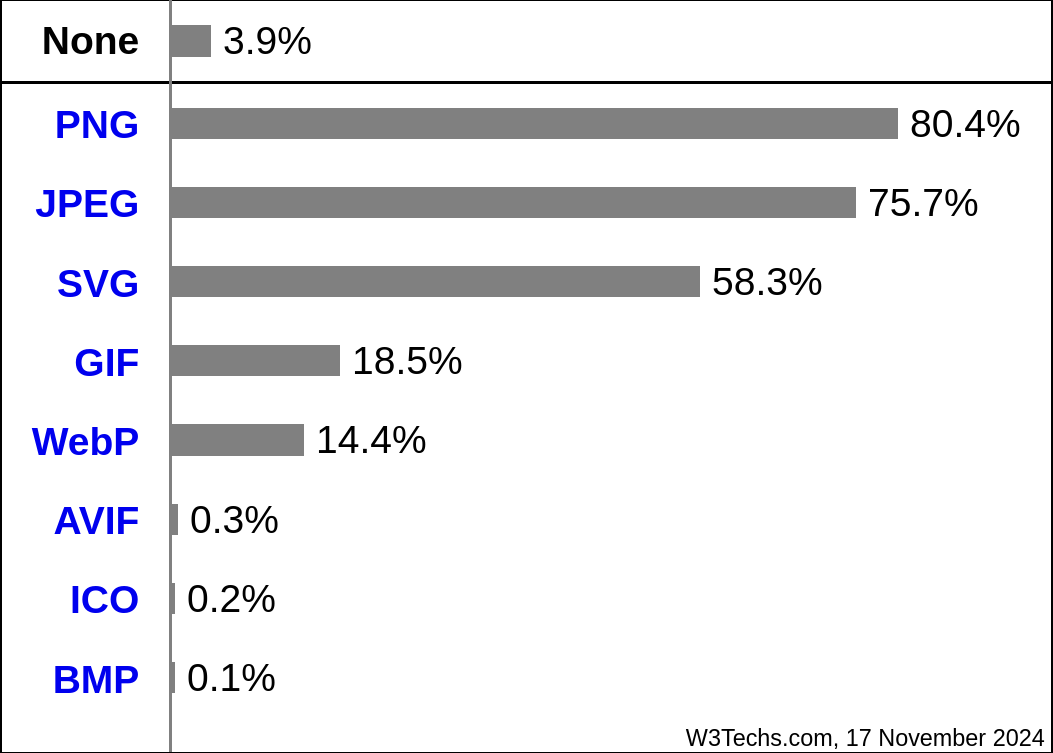
\includegraphics[width=0.4\textwidth]{images/formats}
    \vspace{-10pt}
    \caption{Websites using various image file formats~\cite{img_file_format}}
    \label{fig:file_formats}
\end{wrapfigure}

\subsection{Non-ML Baseline: JPEG}\label{subsec:jpeg}
While much of the current work in realistic high resolution image generation, e.g. \ac{gan} or \ac{vq}, is based on
\ac{dnn}, the field of image compression is well researched both in-, and outside deep architectures~\cite{compression}.
Non-ML approaches are still dominant on the web as can be seen in Figure~\ref{fig:file_formats}.
Due to this prevalence of such approaches, we compare our results to the popular JPEG format for lossy compression.
The algorithm is described by~\cite{jpeg} and can be set to different levels, trading image quality for compression
rate.

\subsection{Autoencoder}\label{subsec:autoencoder}
\begin{wrapfigure}{r}{0.5\textwidth}
    \centering
    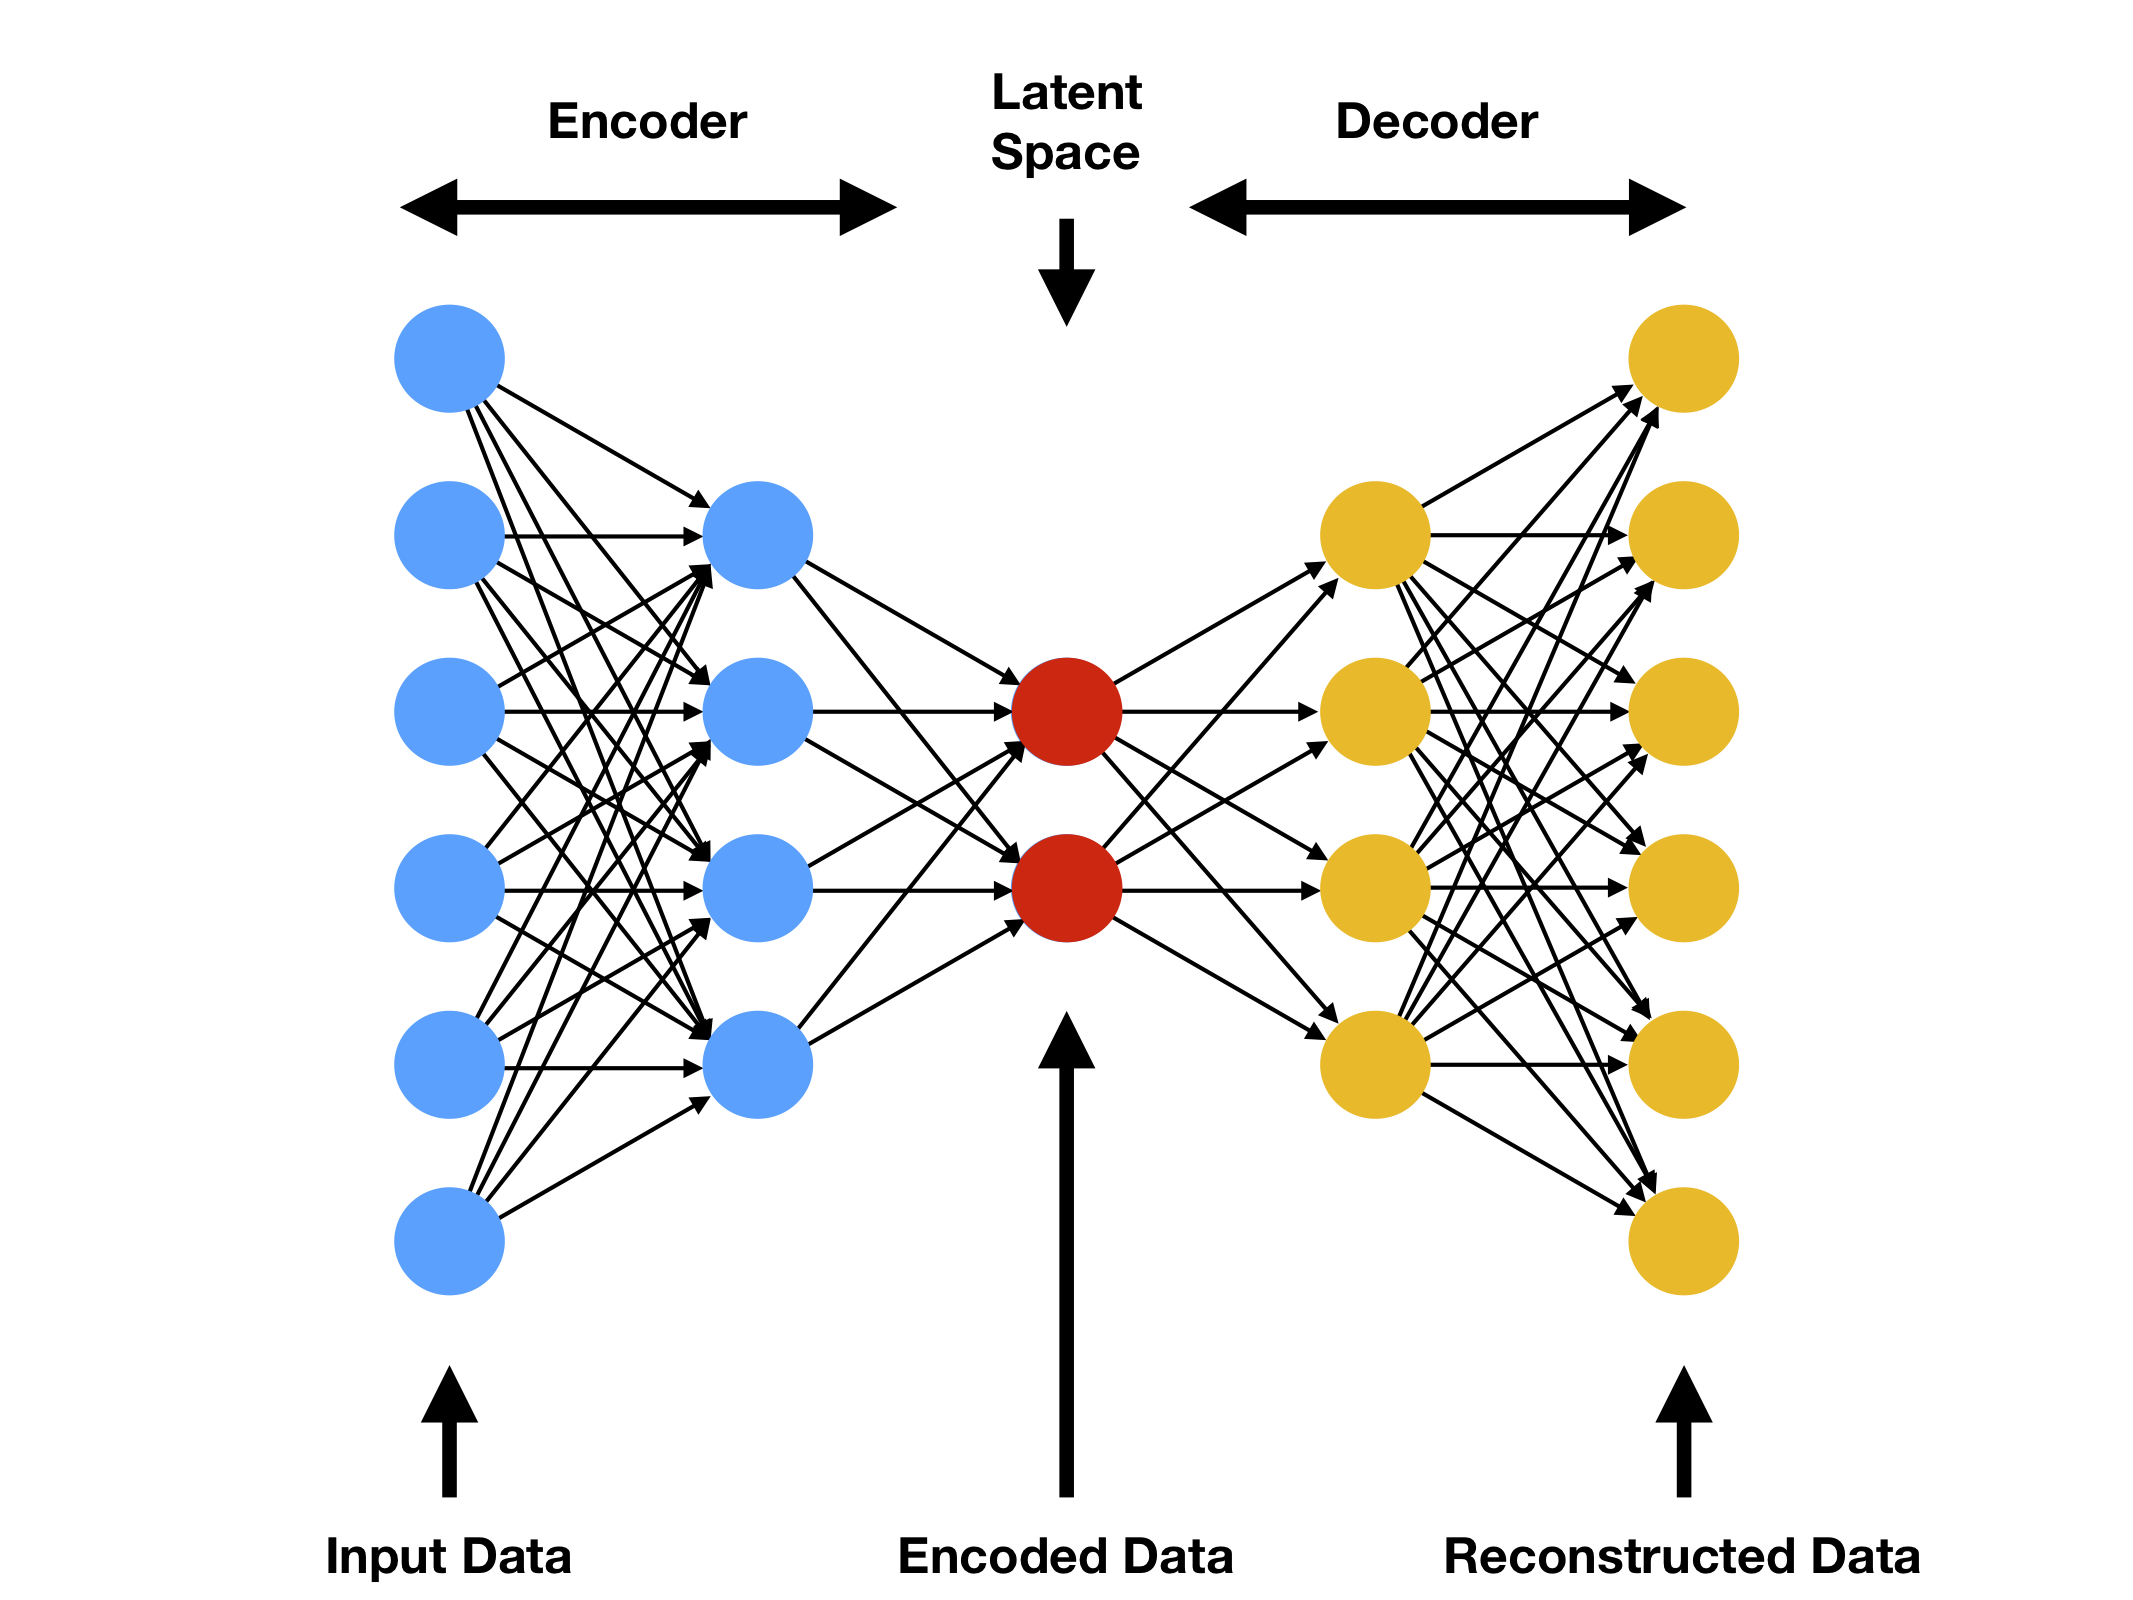
\includegraphics[width=0.5\textwidth]{images/ae}
    \caption{Illustration of a basic \ac{ae} architecture from~\cite{ae_pic}}
    \label{fig:ae}
\end{wrapfigure}

We selected a basic \ac{ae} as our \ac{ml} baseline method for compression because it serves as the foundation
for the original \ac{vae}, which was later extended to the \ac{vq}.

A basic \ac{ae}, as described by~\cite{autoenc} and shown in Figure~\ref{fig:ae}, is a neural network designed to compress and reconstruct data. In our case, the input is an image. During the encoding stage, the network compresses the input data to a lower-dimensional representation using one or more fully connected hidden layers.
The output of this stage is passed to a latent layer, whose dimensionality determines the size of the compressed representation.

The decoding stage, which mirrors the structure of the encoding stage, upsamples the latent representation to reconstruct the original input.
The final output, the reconstruction, has the same shape as the input data, allowing for a direct comparison between the two.

The model can be trained by applying gradient descent on some form of cost function that describes reconstruction error
like \ac{mse}, theoretically pushing the network to encode the information most important to deconstruction in the
latent.

The similarities to \ac{vq} enable highly comparable results, as the \ac{ae} can be adjusted to closely match the
size, training requirements, and inference costs of the \ac{vq}.
In implementing the \ac{ae} baseline, we follow the same architecture as the \ac{vq} wherever feasible.
Specifically, we replace the fully connected layers of the standard \ac{ae} with the downsampling layers and
residual blocks from the \ac{vq} implementation in our reference paper.
This modification is expected to significantly enhance performance, as convolutional \ac{ae}s have been shown to
outperform basic feed-forward \ac{ae}s in image reconstruction tasks, as demonstrated by~\cite{convae}.

\subsection{Variational AE}\label{subsec:variational-ae}
Examining the differences between evolutionary steps towards the \ac{vq} could prove to be valuable
for our understanding of its performance.
Therefore, we also implement a \ac{vae} as our baseline for image generation.
When constructing the neural network, we follow the same paradigm as with the \ac{ae} before, using the same
encoding and decoding layers as far as possible.
The important difference of the VAE is that its encoder outputs a random variable
$\boldsymbol{\hat{z}} \sim \mathcal{N}(\boldsymbol{\mu_\theta}, \text{diag}
(\boldsymbol{\sigma_\theta}))$. $\boldsymbol{\hat{z}}$ is obtained using the
reparameterization trick, which consists in sampling $\boldsymbol{z}
\sim \mathcal{N}(0, I)$ and then computing $\boldsymbol{\hat{z}} =
\boldsymbol{\mu_\theta} + \boldsymbol{z} \odot \boldsymbol{\sigma_\theta}$.
$\boldsymbol{\mu_\theta}$ and $\boldsymbol{\sigma_\theta}$ are deterministic
outputs of the last convolutional layer of the \ac{vae} encoder.
This allows to optimize the model using the ELBO loss which in turn enables us to not only
reconstruct the input, but to learn a posterior distribution $p(x|z)$ while
the encoder $q(z|x)$ tries to be as close as possible to $p(z)$.
Thus enabling us to generate new dataset samples by sampling $z \sim p(z)$ and then feeding
it through the decoder.